\documentclass[a4paper]{article}
\usepackage{ctex}
\usepackage{amsmath, amssymb, amsthm}
\usepackage{float}
\usepackage{graphicx}
\usepackage{geometry}
\usepackage[thehwcnt = 1]{iidef}
\usepackage{enumitem}
\usepackage{listings}
\usepackage{xcolor}

% 设置图片文件夹路径
\graphicspath{{shell vim图片/}}

% 页面边距配置
\geometry{a4paper, top=2.5cm, bottom=2.5cm, left=3cm, right=2.5cm}
% 全局行间距1.2倍
\linespread{1.2}

\thecourseinstitute{中国海洋大学信息科学与工程学部}
\thecoursename{系统开发工具基础}
\theterm{2025年夏季学期}
\hwname{实验报告二}
\slname{\heiti{解}}

\begin{document}
\courseheader
\name{24计算机科学与技术 吴虹霖 \quad 学号: 24020007135}

% ------------------- 第一大板块:Shell 命令 -------------------
\section{一、Shell 命令}
\begin{enumerate}[itemsep=2\parskip, label=实例1.\arabic*]

% 实例1.1:nano文本编辑器写入内容
\item \textbf{nano文本编辑器写入内容}
\begin{description}[
leftmargin=7em,
labelwidth=5em,
labelsep=1em,
itemsep=1\parskip,
align=right
]
\item [\textbf{Q}:] 使用nano文本编辑器创建并编辑一个文件,写入指定内容。
\item [\textbf{A}:] 
1.打开终端,输入 nano example.txt 打开nano编辑器。

2.在编辑器中输入文本内容。

3.按下 Ctrl + O 保存文件,确认文件名后按回车。

4.按下 Ctrl + X 退出nano编辑器。

\begin{figure}[H]
  \centering
  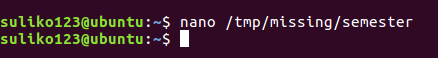
\includegraphics[width=0.8\textwidth]{nano文本编辑器写入内容1.png}
  \caption{nano文本编辑器写入内容1}
  \label{fig:nano1}
\end{figure}

\begin{figure}[H]
  \centering
  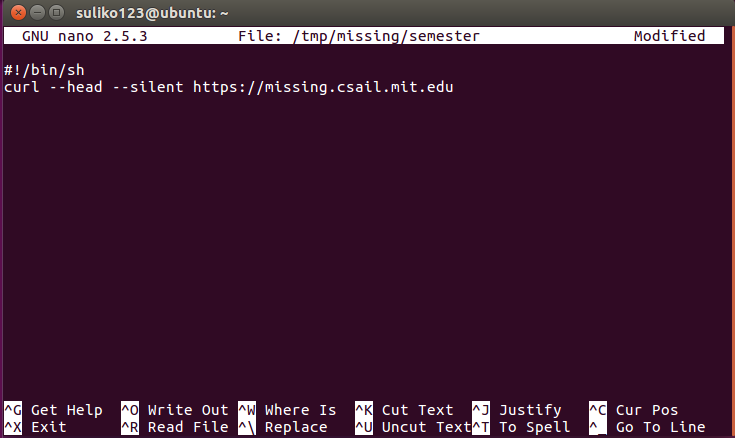
\includegraphics[width=0.8\textwidth]{nano文本编辑器写入内容2.png}
  \caption{nano文本编辑器写入内容2}
  \label{fig:nano2}
\end{figure}
\end{description}

% 实例1.2:touch新建文件
\item \textbf{touch新建文件}
\begin{description}[
leftmargin=7em,
labelwidth=5em,
labelsep=1em,
itemsep=1\parskip,
align=right
]
\item [\textbf{Q}:] 使用touch命令创建一个名为"semester"的空文件。
\item [\textbf{A}:] 
1.在终端中输入以下命令:touch semester

2.使用 ls 命令确认文件已创建。

\begin{figure}[H]
  \centering
  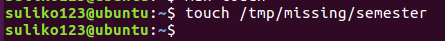
\includegraphics[width=0.8\textwidth]{touch新建semester文件.png}
  \caption{touch新建semester文件}
  \label{fig:touch}
\end{figure}
\end{description}

% 实例1.3:查看touch程序使用手册
\item \textbf{查看touch程序使用手册}
\begin{description}[
leftmargin=7em,
labelwidth=5em,
labelsep=1em,
itemsep=1\parskip,
align=right
]
\item [\textbf{Q}:] 查看touch命令的使用手册。
\item [\textbf{A}:] 
1.在终端中输入:man touch

2.使用方向键浏览,按 q 退出。

\begin{figure}[H]
  \centering
  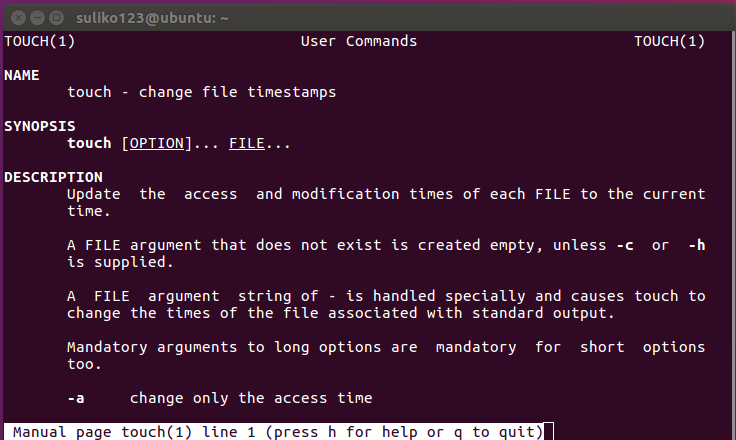
\includegraphics[width=0.8\textwidth]{查看touch程序使用手册.png}
  \caption{查看touch程序使用手册}
  \label{fig:man-touch}
\end{figure}
\end{description}

% 实例1.4:查看当前路径
\item \textbf{查看当前路径}
\begin{description}[
leftmargin=7em,
labelwidth=5em,
labelsep=1em,
itemsep=1\parskip,
align=right
]
\item [\textbf{Q}:] 查看当前所在目录的绝对路径。
\item [\textbf{A}:] 
在终端中输入:pwd

\begin{figure}[H]
  \centering
  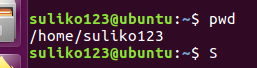
\includegraphics[width=0.8\textwidth]{查看当前路径.png}
  \caption{查看当前路径}
  \label{fig:pwd}
\end{figure}
\end{description}

% 实例1.5:查看权限
\item \textbf{查看权限}
\begin{description}[
leftmargin=7em,
labelwidth=5em,
labelsep=1em,
itemsep=1\parskip,
align=right
]
\item [\textbf{Q}:] 查看当前目录下文件的详细权限信息。
\item [\textbf{A}:] 
在终端中输入:ls -l

\begin{figure}[H]
  \centering
  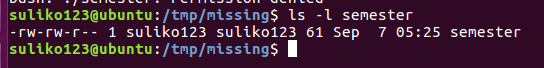
\includegraphics[width=0.8\textwidth]{查看权限.png}
  \caption{查看权限}
  \label{fig:ls-l}
\end{figure}
\end{description}

% 实例1.6:导航文件夹
\item \textbf{导航文件夹}
\begin{description}[
leftmargin=7em,
labelwidth=5em,
labelsep=1em,
itemsep=1\parskip,
align=right
]
\item [\textbf{Q}:] 切换至目标目录。
\item [\textbf{A}:] 
在终端中输入:cd ..

\begin{figure}[H]
  \centering
  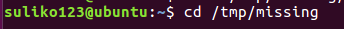
\includegraphics[width=0.8\textwidth]{导航文件夹.png}
  \caption{导航文件夹}
  \label{fig:cd}
\end{figure}
\end{description}

% 实例1.7:执行文件
\item \textbf{执行文件}
\begin{description}[
leftmargin=7em,
labelwidth=5em,
labelsep=1em,
itemsep=1\parskip,
align=right
]
\item [\textbf{Q}:] 尝试执行一个文件。
\item [\textbf{A}:] 
输入文件路径尝试执行,./

\begin{figure}[H]
  \centering
  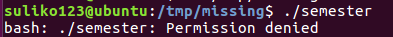
\includegraphics[width=0.8\textwidth]{执行文件.png}
  \caption{执行文件}
  \label{fig:execute}
\end{figure}
\end{description}

% 实例1.8:查看指定目录文件
\item \textbf{查看指定目录文件}
\begin{description}[
leftmargin=7em,
labelwidth=5em,
labelsep=1em,
itemsep=1\parskip,
align=right
]
\item [\textbf{Q}:] 查看指定目录下的文件。
\item [\textbf{A}:] 
使用 ls

\begin{figure}[H]
  \centering
  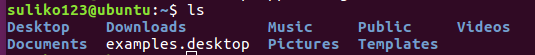
\includegraphics[width=0.8\textwidth]{查看指定目录文件.png}
  \caption{查看指定目录文件}
  \label{fig:ls-dir}
\end{figure}
\end{description}

% 实例1.9:添加权限
\item \textbf{添加权限}
\begin{description}[
leftmargin=7em,
labelwidth=5em,
labelsep=1em,
itemsep=1\parskip,
align=right
]
\item [\textbf{Q}:] 为文件添加执行权限。
\item [\textbf{A}:] 
使用 chmod 命令

\begin{figure}[H]
  \centering
  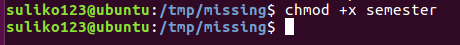
\includegraphics[width=0.8\textwidth]{添加权限.png}
  \caption{添加权限}
  \label{fig:chmod}
\end{figure}
\end{description}

% 实例1.10:新建文件夹
\item \textbf{新建文件夹}
\begin{description}[
leftmargin=7em,
labelwidth=5em,
labelsep=1em,
itemsep=1\parskip,
align=right
]
\item [\textbf{Q}:] 创建一个名为"test\_dir"的目录。
\item [\textbf{A}:] 
使用 mkdir 命令:mkdir test\_dir

\begin{figure}[H]
  \centering
  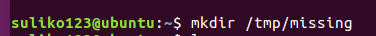
\includegraphics[width=0.8\textwidth]{新建文件夹.png}
  \caption{新建文件夹}
  \label{fig:mkdir}
\end{figure}
\end{description}
\end{enumerate}

% ------------------- 第二大板块:Vim 命令 -------------------
\section{二、Vim 命令}
\begin{enumerate}[itemsep=2\parskip, label=实例2.\arabic*, start=1]

% 实例2.1:创建test文件
\item \textbf{创建test文件}
\begin{description}[
leftmargin=7em,
labelwidth=5em,
labelsep=1em,
itemsep=1\parskip,
align=right
]
\item [\textbf{Q}:] 使用Vim创建并编辑一个名为"test"的文件。
\item [\textbf{A}:] 
输入 vim test.txt

\begin{figure}[H]
  \centering
  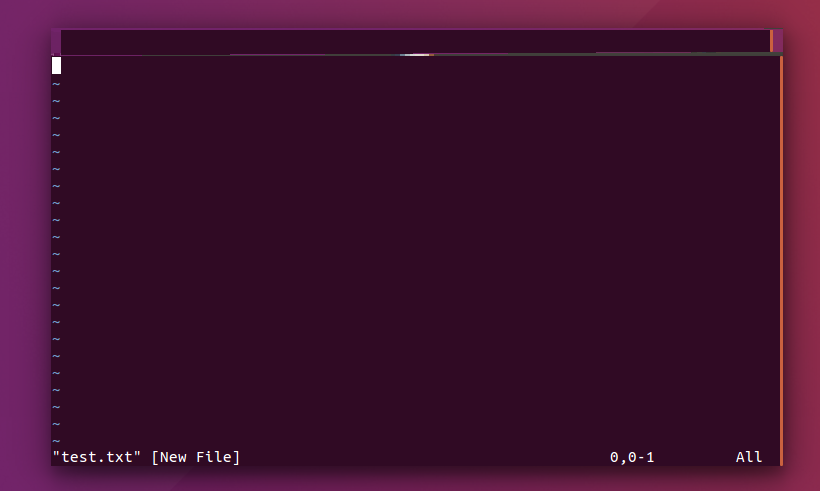
\includegraphics[width=0.8\textwidth]{创建test文件.png}
  \caption{创建test文件}
  \label{fig:vim-create}
\end{figure}
\end{description}

% 实例2.2:查看vim版本
\item \textbf{查看vim版本}
\begin{description}[
leftmargin=7em,
labelwidth=5em,
labelsep=1em,
itemsep=1\parskip,
align=right
]
\item [\textbf{Q}:] 查看当前系统中安装的Vim版本。
\item [\textbf{A}:] 
在终端中输入:vim --version

\begin{figure}[H]
  \centering
  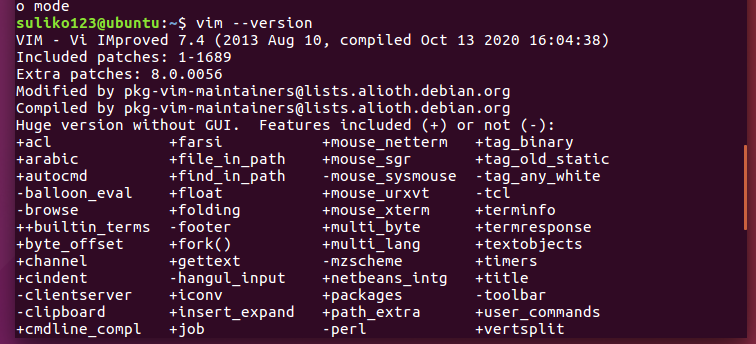
\includegraphics[width=0.8\textwidth]{查看vim版本.png}
  \caption{查看vim版本}
  \label{fig:vim-version}
\end{figure}
\end{description}

% 实例2.3:保存文档
\item \textbf{保存文档}
\begin{description}[
leftmargin=7em,
labelwidth=5em,
labelsep=1em,
itemsep=1\parskip,
align=right
]
\item [\textbf{Q}:] 在Vim中编辑文件后保存并退出。
\item [\textbf{A}:] 
在命令模式下输入::wq

\begin{figure}[H]
  \centering
  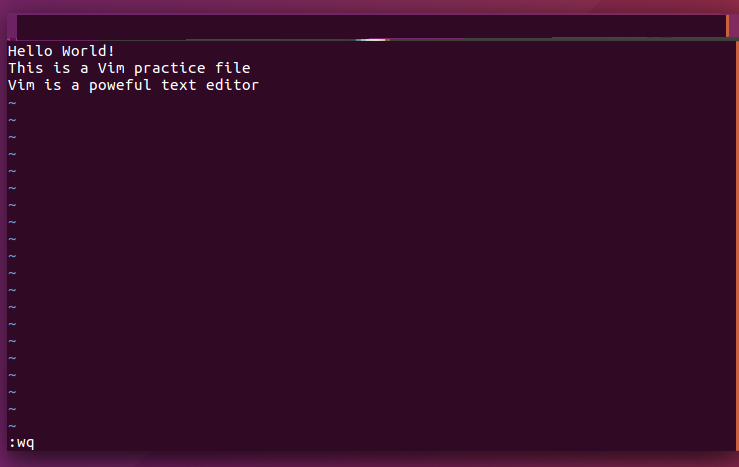
\includegraphics[width=0.8\textwidth]{保存文档.png}
  \caption{保存文档}
  \label{fig:vim-save}
\end{figure}
\end{description}

% 实例2.4:部分替换
\item \textbf{部分替换}
\begin{description}[
leftmargin=7em,
labelwidth=5em,
labelsep=1em,
itemsep=1\parskip,
align=right
]
\item [\textbf{Q}:] 使用Vim替换文件中部分文本内容。
\item [\textbf{A}:] 
在命令模式下输入::s/old/new/g

\begin{figure}[H]
  \centering
  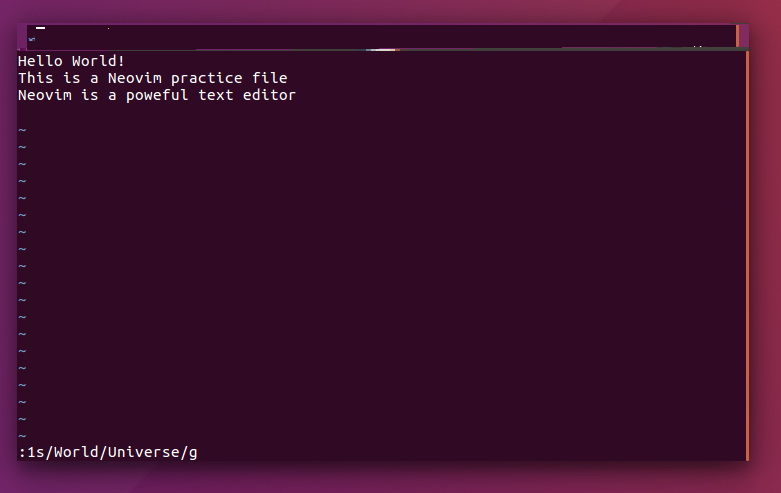
\includegraphics[width=0.8\textwidth]{部分替换.png}
  \caption{部分替换}
  \label{fig:vim-replace}
\end{figure}
\end{description}

% 实例2.5:查找
\item \textbf{查找}
\begin{description}[
leftmargin=7em,
labelwidth=5em,
labelsep=1em,
itemsep=1\parskip,
align=right
]
\item [\textbf{Q}:] 在Vim中查找指定字符串。
\item [\textbf{A}:] 
在命令模式下输入:/要查找的字符串

\begin{figure}[H]
  \centering
  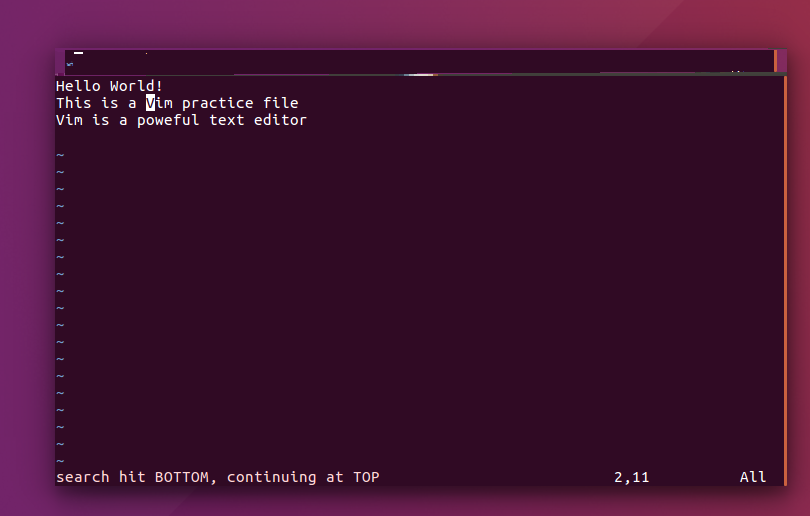
\includegraphics[width=0.8\textwidth]{查找.png}
  \caption{查找}
  \label{fig:vim-search}
\end{figure}
\end{description}

% 实例2.6:撤销上一步操作
\item \textbf{撤销上一步操作}
\begin{description}[
leftmargin=7em,
labelwidth=5em,
labelsep=1em,
itemsep=1\parskip,
align=right
]
\item [\textbf{Q}:] 在Vim中撤销上一步编辑操作。
\item [\textbf{A}:] 
在命令模式下按 u。

\begin{figure}[H]
  \centering
  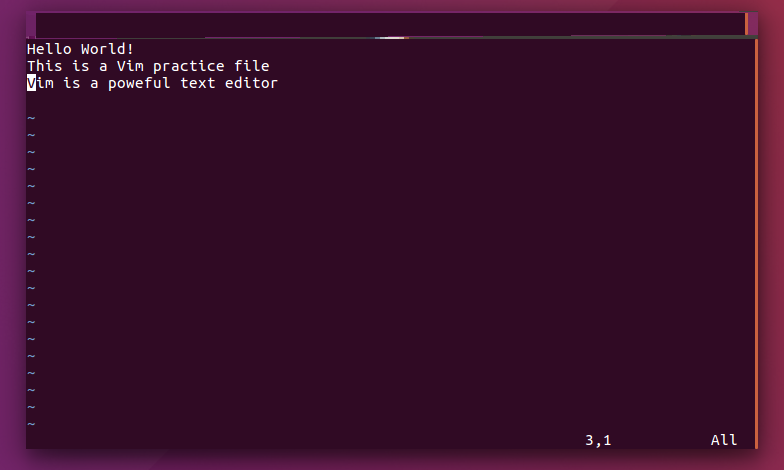
\includegraphics[width=0.8\textwidth]{撤销上一步操作.png}
  \caption{撤销上一步操作}
  \label{fig:vim-undo}
\end{figure}
\end{description}

% 实例2.7:分割窗口
\item \textbf{分割窗口}
\begin{description}[
leftmargin=7em,
labelwidth=5em,
labelsep=1em,
itemsep=1\parskip,
align=right
]
\item [\textbf{Q}:] 在Vim中水平分割窗口。
\item [\textbf{A}:] 
在命令模式下输入::split

\begin{figure}[H]
  \centering
  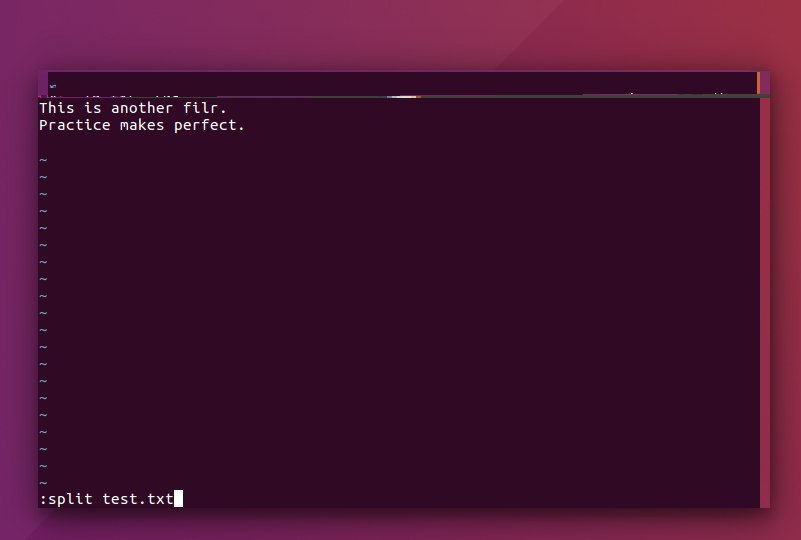
\includegraphics[width=0.8\textwidth]{分割窗口.png}
  \caption{分割窗口}
  \label{fig:vim-split}
\end{figure}
\end{description}

% 实例2.8:复制粘贴
\item \textbf{复制粘贴}
\begin{description}[
leftmargin=7em,
labelwidth=5em,
labelsep=1em,
itemsep=1\parskip,
align=right
]
\item [\textbf{Q}:] 在Vim中复制一行并粘贴。
\item [\textbf{A}:] 
将光标移至要复制的行。按 yy 复制该行。移动光标至目标位置,按 p 粘贴。

\begin{figure}[H]
  \centering
  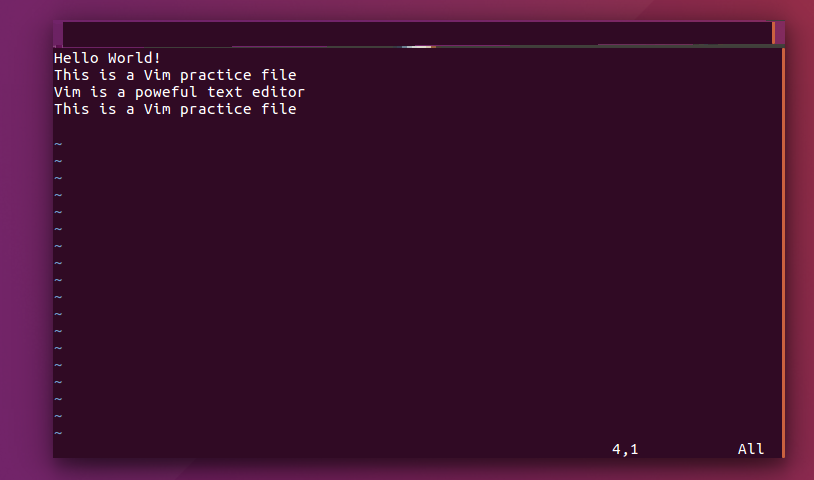
\includegraphics[width=0.8\textwidth]{复制与粘贴.png}
  \caption{复制与粘贴}
  \label{fig:vim-copy-paste}
\end{figure}
\end{description}

% 实例2.9:录制并应用宏
\item \textbf{录制并应用宏}
\begin{description}[
leftmargin=7em,
labelwidth=5em,
labelsep=1em,
itemsep=1\parskip,
align=right
]
\item [\textbf{Q}:] 在Vim中录制宏并重复执行。
\item [\textbf{A}:] 
按 q 加一个寄存器(如 q)开始录制。执行一系列操作。按 q 结束录制。按 @q 执行宏。

\begin{figure}[H]
  \centering
  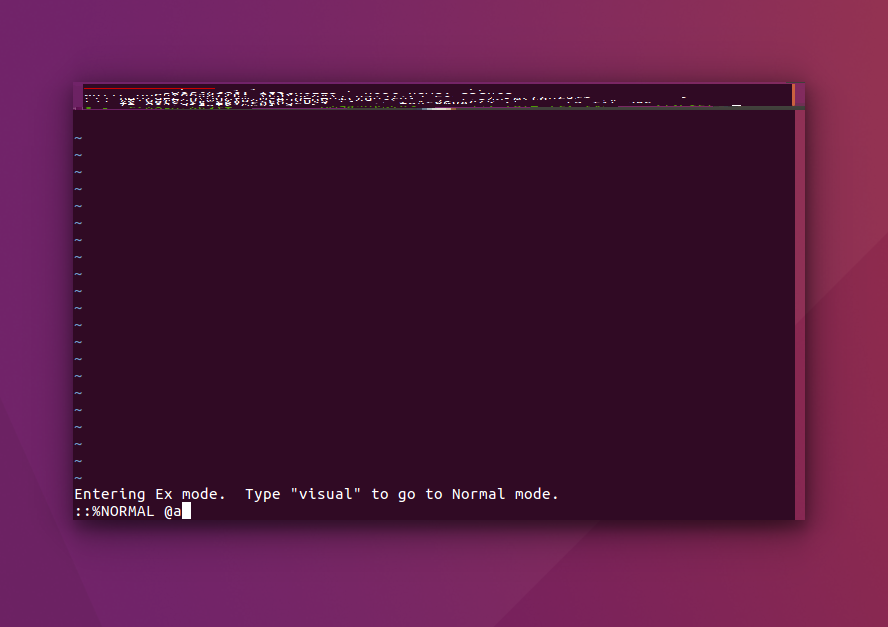
\includegraphics[width=0.8\textwidth]{录制并应用宏.png}
  \caption{录制并应用宏}
  \label{fig:vim-macro}
\end{figure}
\end{description}

% 实例2.10:全局替换
\item \textbf{全局替换}
\begin{description}[
leftmargin=7em,
labelwidth=5em,
labelsep=1em,
itemsep=1\parskip,
align=right
]
\item [\textbf{Q}:] 在Vim中对整个文件进行字符串替换。
\item [\textbf{A}:] 
在命令模式下输入::\%s/old/new/g

\begin{figure}[H]
  \centering
  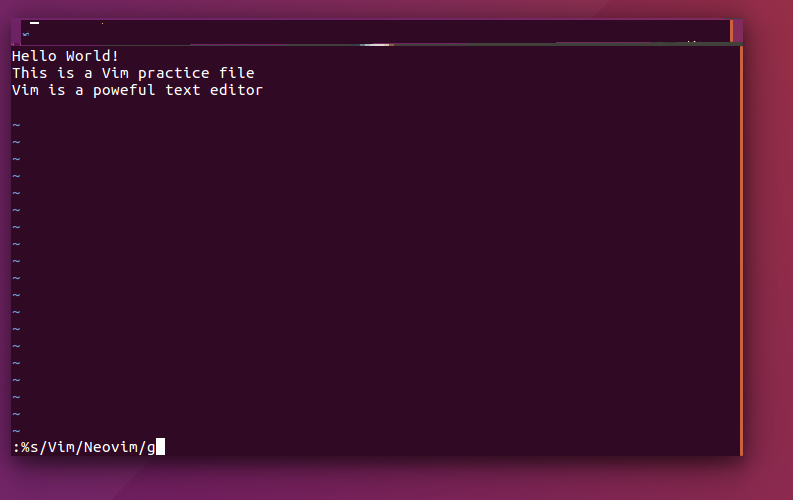
\includegraphics[width=0.8\textwidth]{全局替换.png}
  \caption{全局替换}
  \label{fig:vim-global-replace}
\end{figure}
\end{description}
\end{enumerate}

% 添加到 \end{document} 前
\section*{个人心得}
通过本次实验,我系统性地学习了 Shell 和 Vim 两大核心工具的基本操作与高级功能。在 Shell 部分,掌握了文件管理、权限设置、进程执行等关键命令,理解了命令行环境下的高效工作流。Vim 部分则从基础编辑入手,逐步练习了文本替换、宏录制、窗口分割等进阶操作,显著提升了代码和文档的编辑效率。

实验过程中,我尤其体会到理论与实践结合的重要性:仅阅读手册不足以熟练掌握工具,唯有反复实践才能内化技能。此外,遇到权限问题、命令失败等情况时,通过查阅文档和调试解决了问题,增强了自主解决问题的能力。

本次实验不仅巩固了系统开发工具的基础知识,也为后续的编程和系统管理工作奠定了扎实基础。未来我将进一步探索 Shell 脚本编写和 Vim 定制化配置,以提升自动化处理与个性化开发环境的构建能力。

\end{document}